\documentclass[12pt,a4paper]{article}
\usepackage[utf8]{inputenc}
\usepackage[T1]{fontenc}
\usepackage[brazil]{babel}
\usepackage{geometry}
\usepackage{setspace}
\usepackage{graphicx}
\usepackage{float}
\geometry{margin=2.5cm}
\setstretch{1.15}
\setlength{\parindent}{0pt}
\setlength{\parskip}{0.35em}

\begin{document}

\begin{center}
\textbf{Ministério da Educação}\\
\textbf{Universidade Tecnológica Federal do Paraná -- Campus Pato Branco}\\
\textbf{Departamento Acadêmico de Informática}\\[0.5em]
\textbf{Disciplina: Redes de Computadores} \hfill \textbf{Prof. Dr. Eden Dosciatti}

\vspace{1.2em}
\Large\textbf{Atividade Avaliativa 4}
\end{center}

\vspace{1em}
\noindent\textbf{Nome:} Pedro Mariano dos Santos \hfill \textbf{RA:} 2562790

\vspace{1em}

\section*{Cenário 1: Implementação de Infraestrutura (Do Zero)}

A topologia foi montada com roteador, switch, três servidores dedicados (Web, DHCP e DNS) e seis estações com IP dinâmico. O segmento utilizado foi \texttt{192.168.22.0/24}, com gateway \texttt{192.168.22.1}.

\subsection*{Resultados dos testes (Cenário 1)}

\begin{figure}[H]
\centering
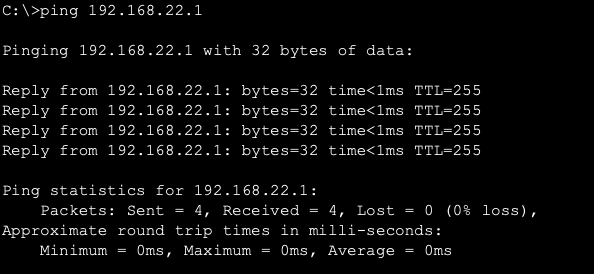
\includegraphics[width=0.95\linewidth]{assets/c1_pc0_ping_gateway.png}
\caption{Teste de conectividade IP entre estação e gateway (sucesso).}
\end{figure}

\begin{figure}[H]
\centering
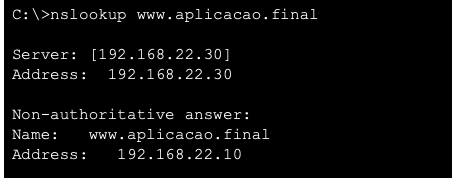
\includegraphics[width=0.95\linewidth]{assets/c1_pc4_nslookup.png}
\caption{Resolução de nomes por \texttt{nslookup} no PC4 (sucesso).}
\end{figure}

\begin{figure}[H]
\centering
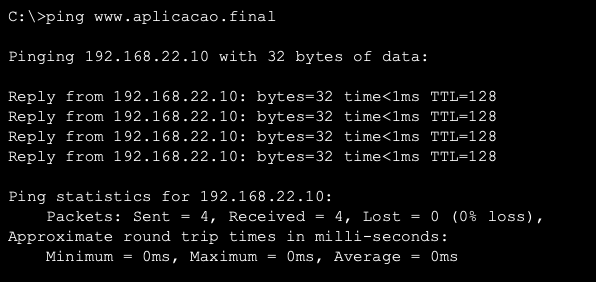
\includegraphics[width=0.95\linewidth]{assets/c1_pc0_ping_dominio.png}
\caption{Teste DNS no PC0 com \texttt{ping www.aplicacao.final} (sucesso).}
\end{figure}

\begin{figure}[H]
\centering
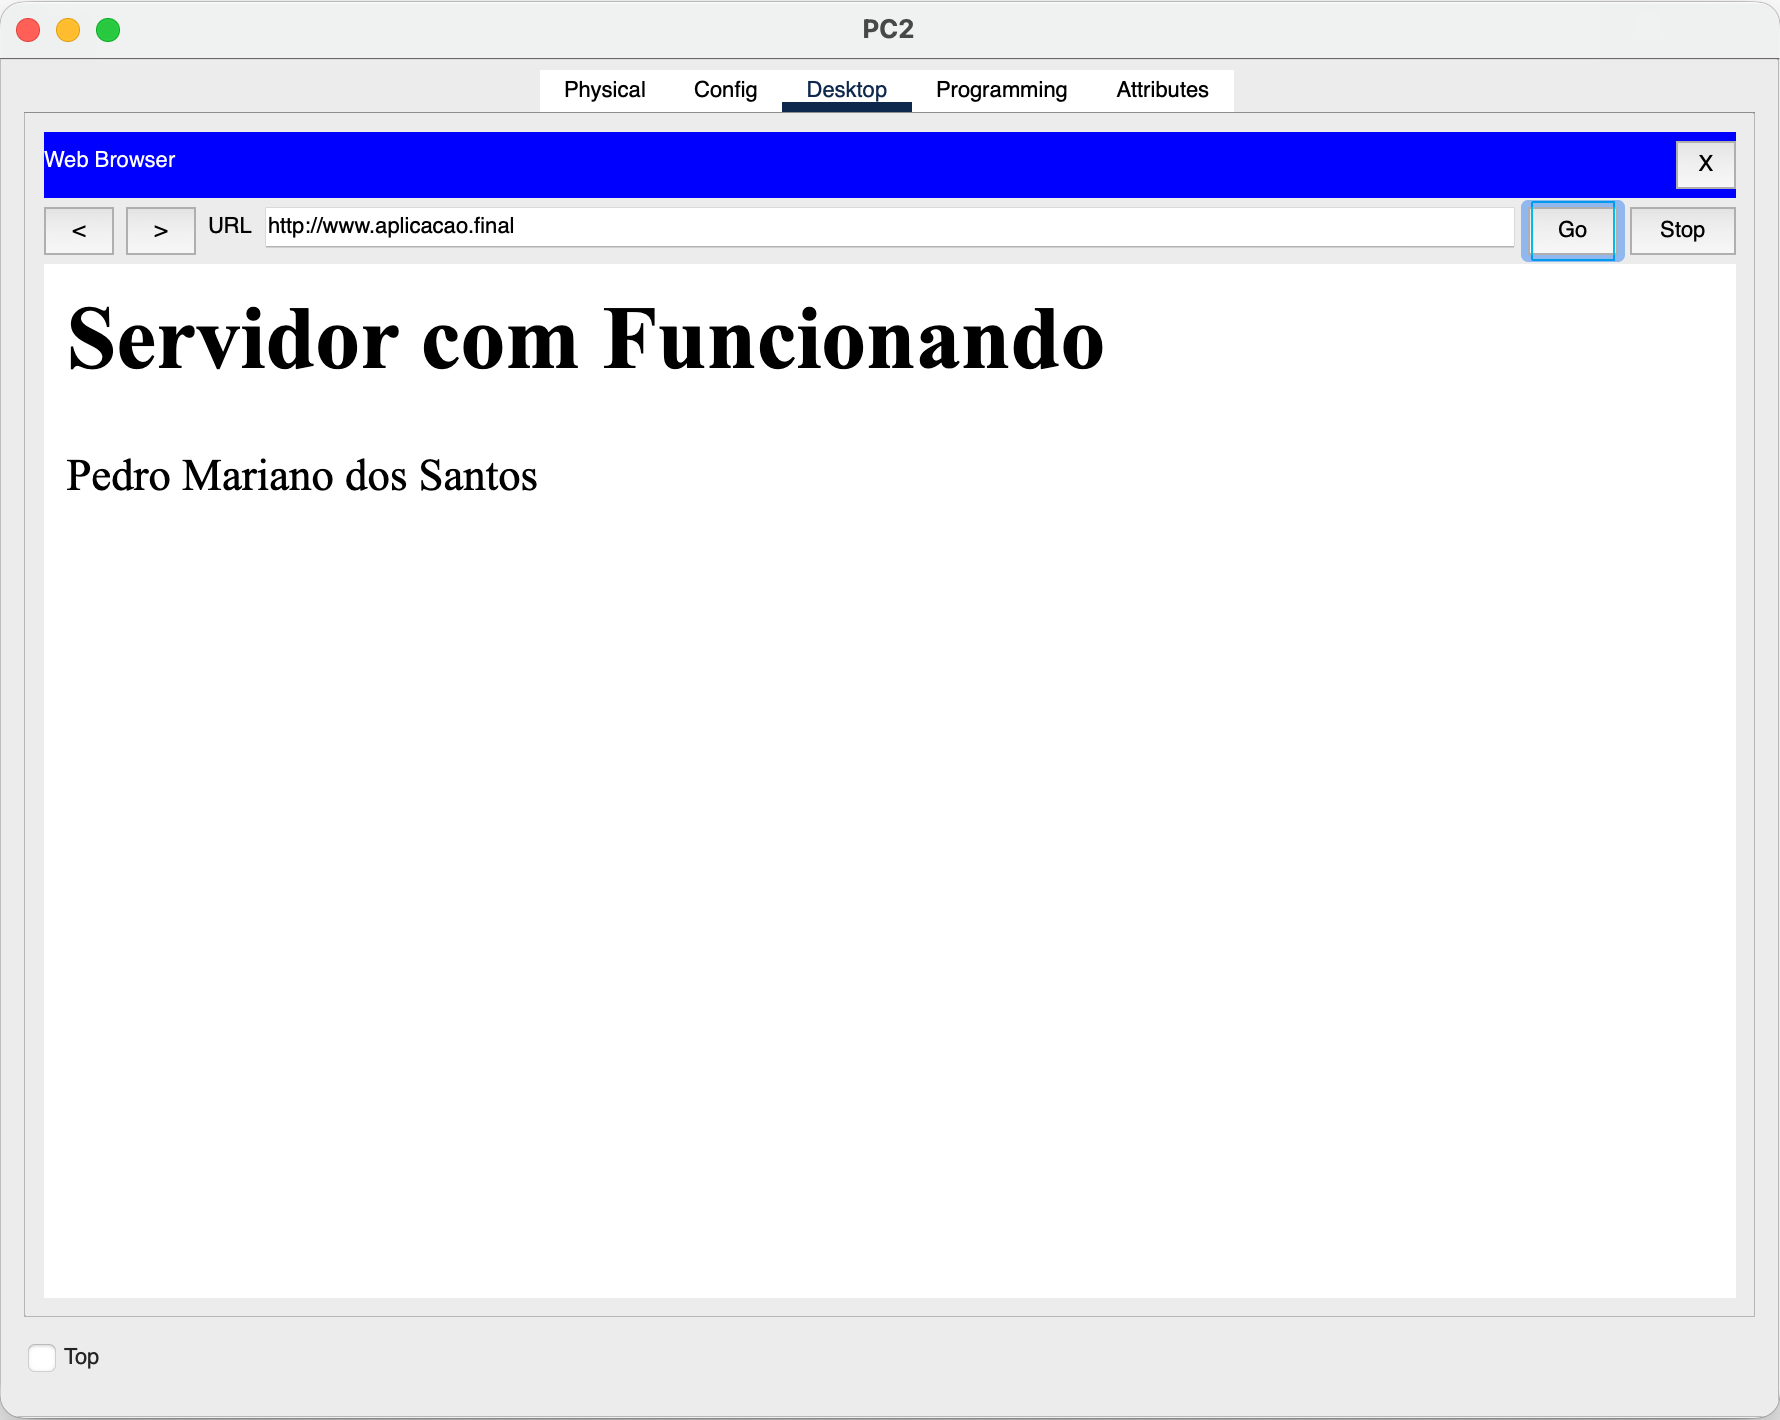
\includegraphics[width=0.95\linewidth]{assets/c1_pc2_browser.png}
\caption{Acesso HTTP no navegador do PC2 (renderização da aplicação).}
\end{figure}

\subsection*{Respostas às questões do Cenário 1}

\begin{enumerate}
\item \textbf{Qual IP o computador PC0 recebeu? Veio do pool?}\\
PC0 recebeu \texttt{192.168.22.170}. Sim, veio do pool DHCP iniciado em \texttt{192.168.22.150}.

\item \textbf{Qual servidor forneceu esse IP?}\\
O IP foi fornecido pelo servidor DHCP em \texttt{192.168.22.20}.

\item \textbf{Qual IP resolve o nome \texttt{www.aplicacao.final}?}\\
Resolve para \texttt{192.168.22.10}.

\item \textbf{O que acontece se o DNS estiver errado?}\\
A resolução de nomes falha e os clientes não conseguem acessar a aplicação pelo domínio, mesmo que o servidor esteja ativo por IP.

\item \textbf{Qual protocolo é usado no navegador?}\\
HTTP.

\item \textbf{Qual porta o HTTP utiliza?}\\
Porta 80/TCP.

\item \textbf{O que acontece se o HTTP estiver desligado?}\\
O domínio pode resolver normalmente, mas o acesso à página no navegador falha, pois o serviço web não está disponível.

\item \textbf{Qual a função do gateway?}\\
Encaminhar pacotes para redes externas ao segmento local, atuando como próximo salto para o tráfego dos hosts.
\end{enumerate}

\newpage
\section*{Cenário 2: O Desafio do Administrador (Troubleshooting)}

No cenário de erro, a topologia possui um único servidor concentrando serviços. A análise da configuração inicial permitiu identificar inconsistências de DHCP, DNS e HTTP, causando falha de acesso ao domínio \texttt{www.aplicacao.erros}.

\subsection*{Erros encontrados}
\begin{enumerate}
\item Serviço HTTP do servidor estava desligado.
\item Registro DNS cadastrado com nome incorreto (\texttt{www.aplicacao.eros}).
\item Registro DNS apontando para IP incorreto (\texttt{172.100.22.100} em vez de \texttt{172.100.22.10}).
\item DHCP com \textit{default gateway} incorreto (\texttt{172.100.22.11}).
\item DHCP com DNS server incorreto (\texttt{172.100.22.100}).
\item Faixa/política de usuários DHCP restritiva para a quantidade de estações.
\end{enumerate}

\subsection*{Correções realizadas}
\begin{enumerate}
\item Ativação do serviço HTTP no servidor.
\item Correção do registro DNS para \texttt{www.aplicacao.erros}.
\item Correção do endereço do registro A para \texttt{172.100.22.10}.
\item Ajuste do gateway DHCP para \texttt{172.100.22.1}.
\item Ajuste do DNS distribuído pelo DHCP para \texttt{172.100.22.10}.
\item Renovação de endereçamento dos clientes DHCP após as correções.
\item Manutenção do PC2 com endereçamento estático, conforme enunciado.
\end{enumerate}

\subsection*{Resultados dos testes (Cenário 2)}

\begin{figure}[H]
\centering
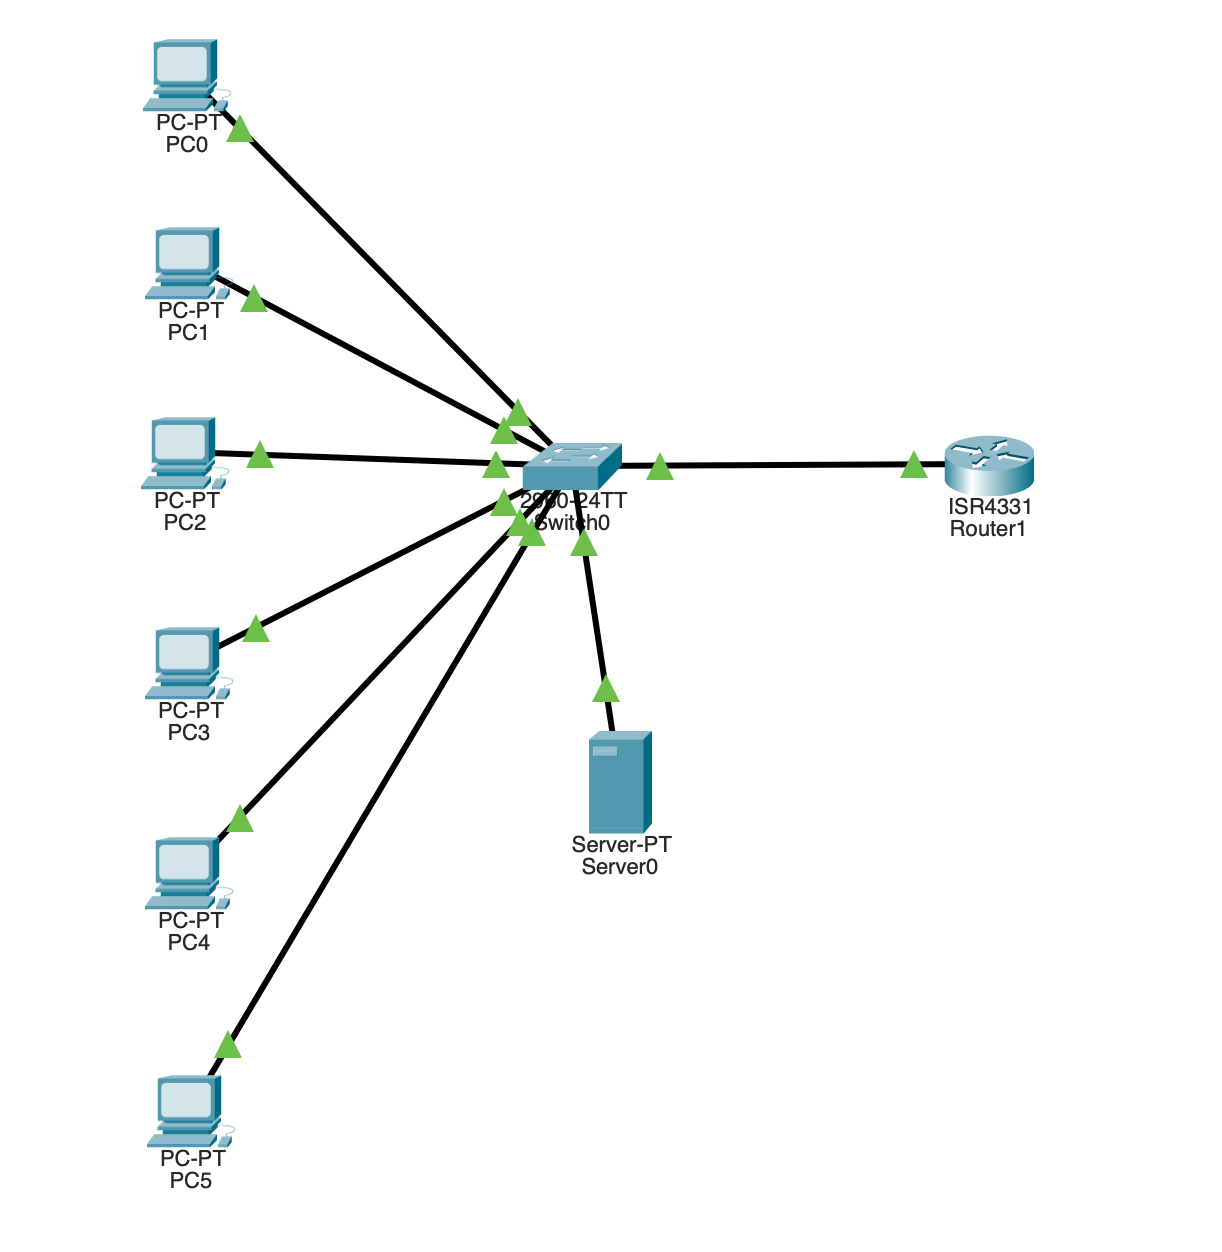
\includegraphics[width=0.85\linewidth]{assets/c2_topologia.png}
\caption{Topologia final do cenário 2 após as correções.}
\end{figure}

\begin{figure}[H]
\centering
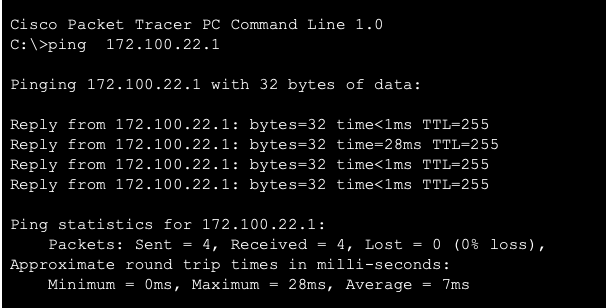
\includegraphics[width=0.95\linewidth]{assets/c2_ping_gateway.png}
\caption{Conectividade IP entre estação e gateway (sucesso).}
\end{figure}

\begin{figure}[H]
\centering
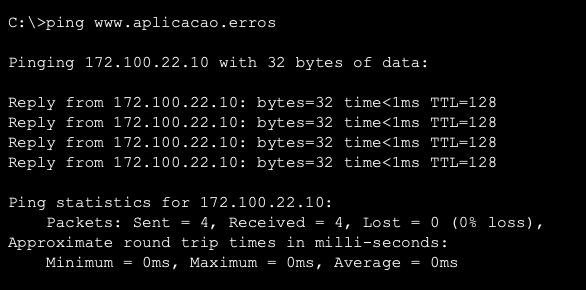
\includegraphics[width=0.95\linewidth]{assets/c2_ping_dominio_pc0.png}
\caption{Teste DNS no PC0 com \texttt{ping www.aplicacao.erros} (sucesso).}
\end{figure}

\begin{figure}[H]
\centering
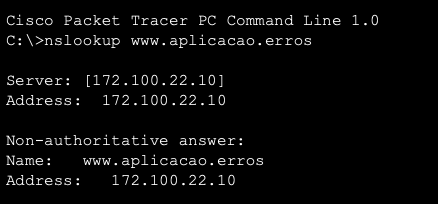
\includegraphics[width=0.95\linewidth]{assets/c2_pc4_nslookup.png}
\caption{Resolução de nomes no PC4 com \texttt{nslookup www.aplicacao.erros} (sucesso).}
\end{figure}

\begin{figure}[H]
\centering
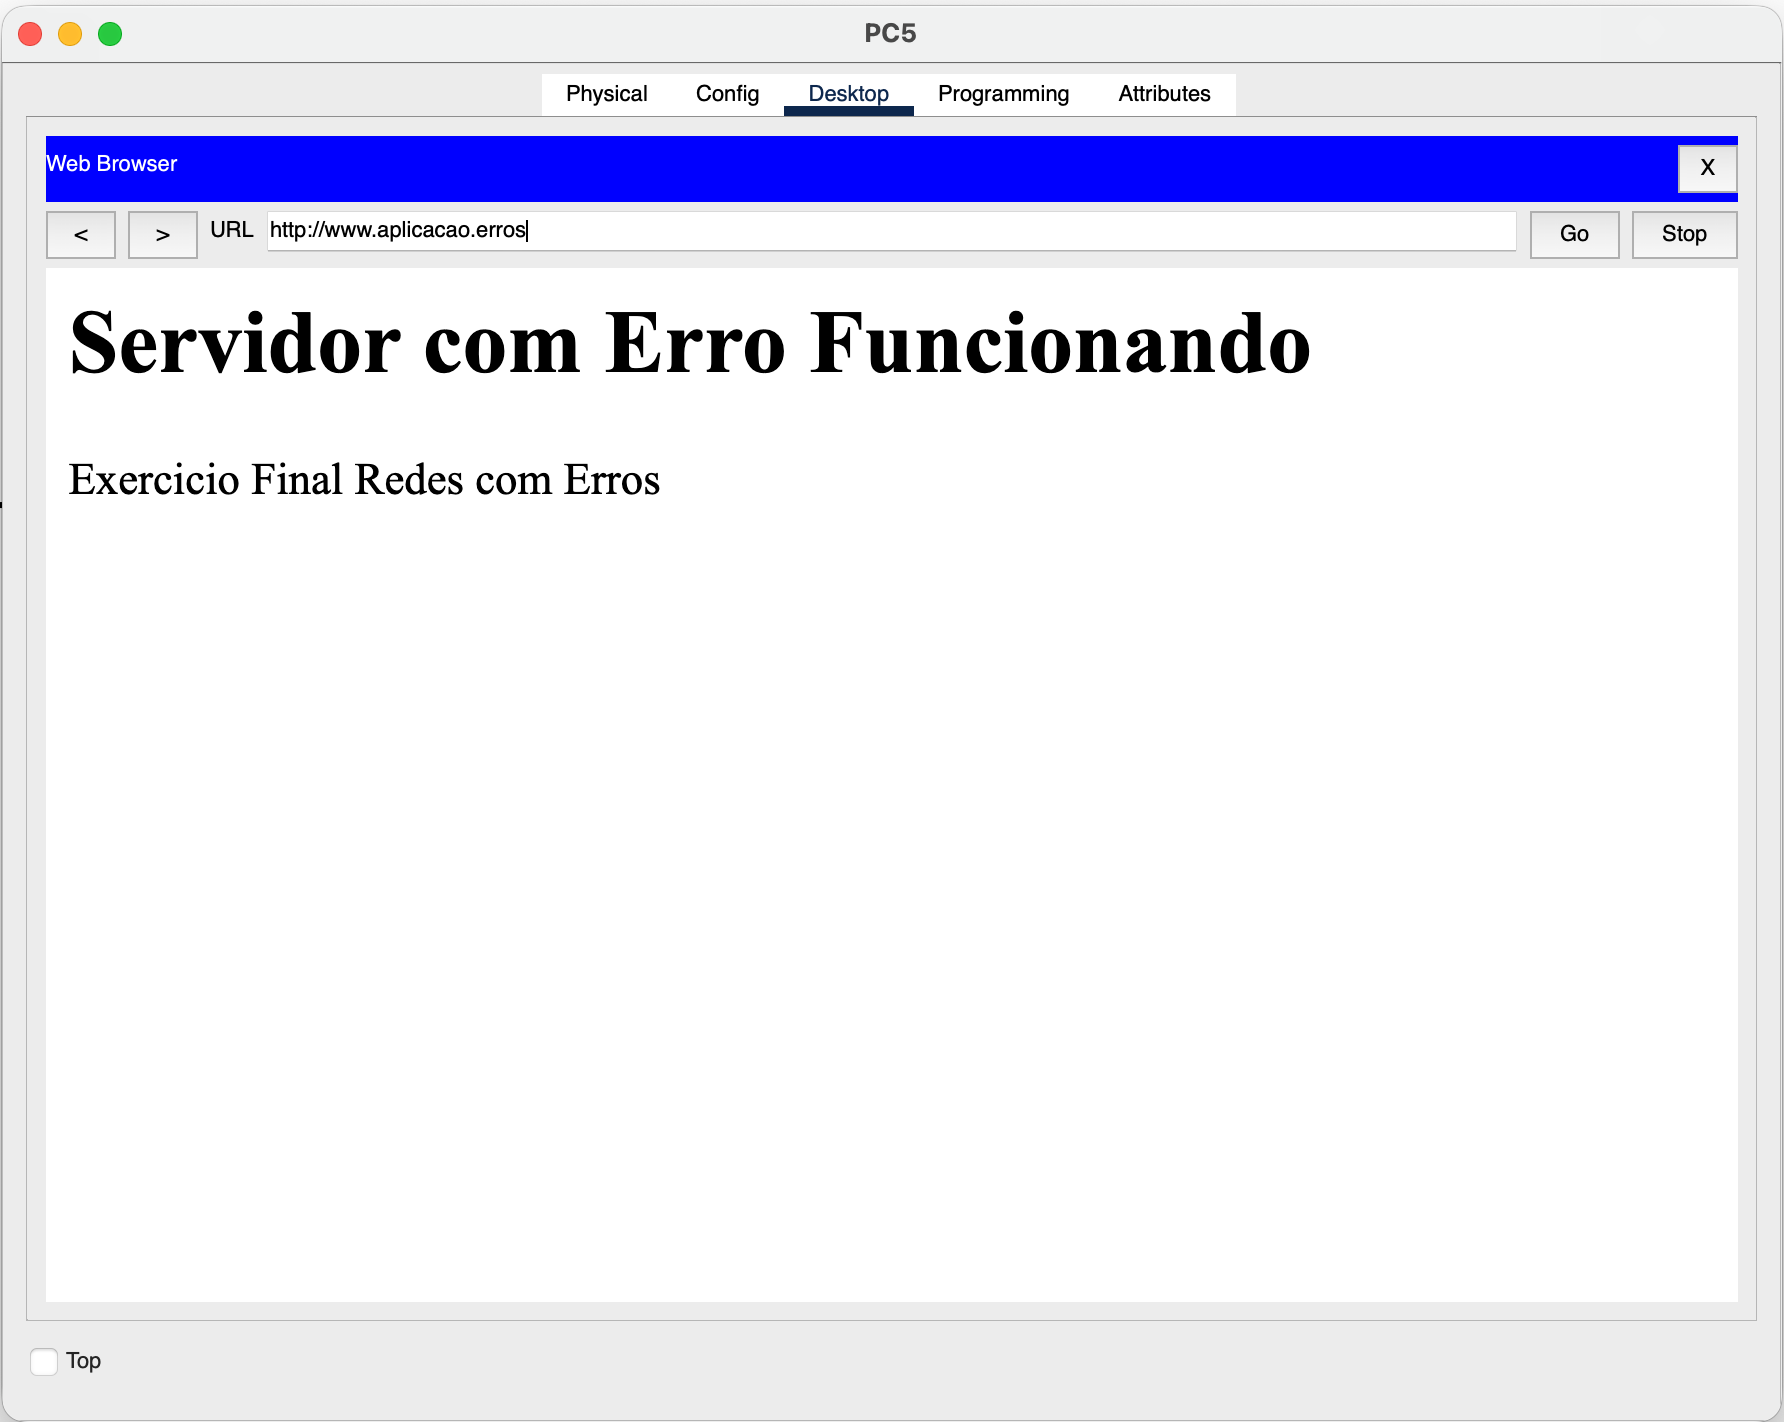
\includegraphics[width=0.95\linewidth]{assets/c2_pc5_browser.png}
\caption{Acesso à aplicação no navegador do PC5 (sucesso).}
\end{figure}

\begin{figure}[H]
\centering
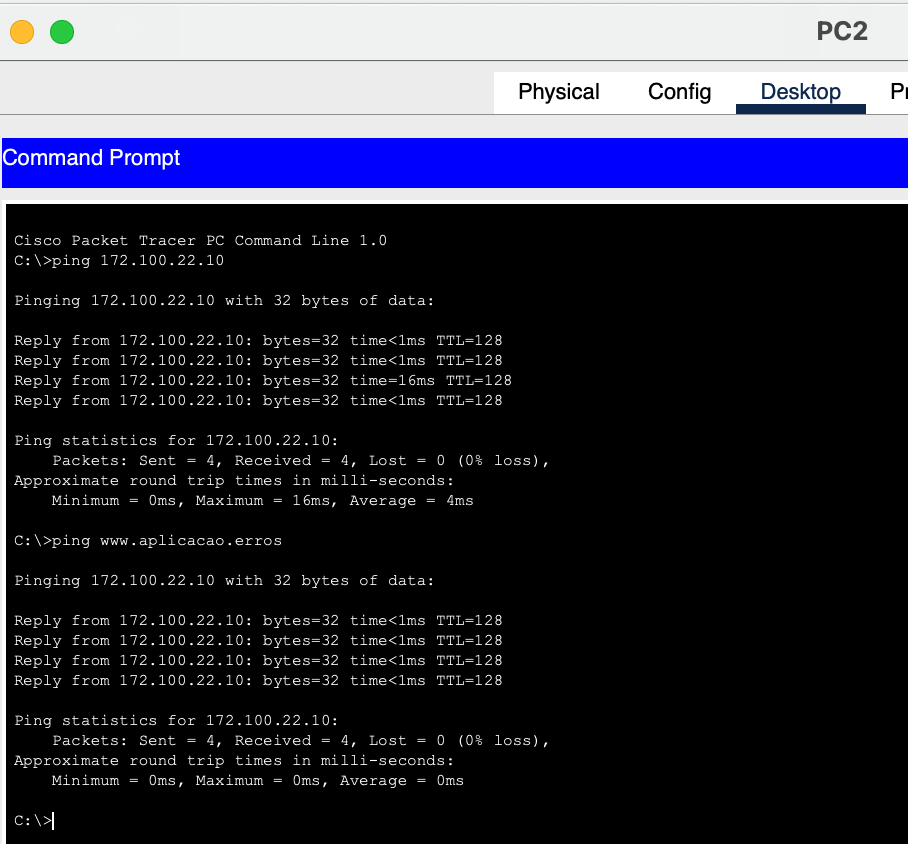
\includegraphics[width=0.95\linewidth]{assets/c2_pc2_pings.png}
\caption{No PC2 (estático): \texttt{ping 172.100.22.10} e \texttt{ping www.aplicacao.erros} com sucesso.}
\end{figure}

\end{document}
